\section{Transfer to dense prediction: More results and addition details.}

\subsection{Semantic segmentation: frozen \textit{versus} fine-tuning.}

\label{app:semantic_segmentation}
In this experiment, we evaluate the effect of fine-tuning \textit{versus} freezing the \chonk backbone when transferring to semantic segmentation.
The results are shown in \cref{tab:semseg_frozen_finetune}.
We observe that for the linear decoder fine-tuning results in much better performance than using frozen features.
For the UperNet decoder, however, the gap between fine-tuning and freezing the backbone is much smaller.
This can be explained by the fact that UperNet has $\sim870$ times more parameters than the linear model.
\cref{fig:dense_prediction} shows qualitative results using Upernet.

\begin{table}[h]
    \caption{
      % \faLock \faLockOpen - these symbols were only used in this one table, so removing these symbols felt more consistent; please add back if they are critical
      {Frozen \textit{versus} fine-tuning transfer of \chonk to semantic segmentation.} 
We report mean IoU on the validation set of 3 popular datasets, namely ADE20k (``A-150'')~\citep{zhou2017scene}, Pascal Context (``P-60'')~\citep{mottaghi2014role}, Pascal VOC and (``P-20'')~\citep{everingham2010pascal}, for different protocols:
(i) frozen \textit{versus} finetuned backbone;
(ii) linear~\citep{strudel2021segmenter} \textit{versus} UperNet~\citep{xiao2018unified} decoder.
}
\centering
%   \setlength{\tabcolsep}{4.5pt}
%   \resizebox{\columnwidth}{!}{%
    \begin{tabular}{@{} l c ccc c ccc @{}}
      \toprule
      Decoder && \multicolumn{3}{c}{Linear} && \multicolumn{3}{c}{UperNet} \\
      % && \multicolumn{3}{c}{Linear~\citet{strudel2021segmenter}} && \multicolumn{3}{c}{UperNet~\citet{xiao2018unified}} \\
\cmidrule{3-5}\cmidrule{7-9}
	      Dataset && A-150 & P-60 & P-20 && A-150 & P-60 & P-20 \\
      \midrule
      \chonk frozen && 34.6 & 38.6 & 65.0 && 52.7 & 58.7 & 78.7 \\
      \chonk fine-tuned\hspace{-1em} && 54.9 & 61.6 & 79.0 && 55.3 & 62.3 & 80.1\\
      \bottomrule
 \end{tabular}
%  }
    \label{tab:semseg_frozen_finetune}
\end{table}




\subsection{Monocular Depth Estimation}
\label{app:de}

\subsubsection{Dataset}

We pre-process Waymo Open video and LiDAR data to obtain RGB frames and associated sparse depth images. The camera frames are extracted from the front-facing camera mounted on the vehicle, while the sparse depth images are obtained by projecting the LiDAR point cloud of a single time step onto the camera frame. We use the camera and LiDAR calibration parameters to compute the distance of each LiDAR point to the camera. For training, we normalize the depth targets using a $\mathrm{log}(1+x)$ transformation; we undo this transformation for metric computation. As the signal is sparse, we mask out any pixels in the depth image for which there is no signal during loss computation.
We evaluate on the first 5120 validation set frames from the front facing camera.

We sub-sample videos to 5 fps, and crop and resize frames to $224\times224$ resolution (both RGB inputs and depth targets). The LiDAR projection is done after cropping and resizing, to retain a high-quality signal. For ViT-L, we upscale the RGB input frames to $256\times256$ resolution to account for the larger patch size, while keeping the same information content as for ViT-e and ViT-22B, which both use a patch size of 14. For evaluation frames, we use a simple center-crop. For training, we use Inception-style~\citep{szegedy2015going} random-resized crops as our only form of data augmentation. We ensure that at least $20\%$ of the original frame is retained after cropping.

For efficiency reasons, we pre-compute ViT-22B feature maps for 1,024,000 randomly sampled and augmented frames from the training set, which amounts to approx.~6.4 epochs of training data. When training the decoder, we iterate over these pre-computed feature maps in random order, irrespective of the number of training steps used. We follow the same protocol for all compared models.

\subsubsection{Decoder Architectures}

\paragraph{Dense Prediction Transformer.}

We largely follow the design of~\citep{ranftl2021vision}, using four reassemble and fusion blocks that processes the $16\times16$ ViT feature map at $(4\times4)$, $(8\times8)$, $(16\times16)$, and $(32\times32)$ spatial resolutions.
We use $64$ features at each stage and thus can omit the $1\times1$ projection convolution in the fusion block. 
The final fusion stage feeds into a monocular depth estimation head, where we use the default $128$ features and adjust the final re-sampling stage to yield the desired resolution of $224\times224$.
Similar to~\citep{ranftl2021vision}, we do not consider dropout or batchnorm for depth estimation.

For efficiency purposes we reuse the same $16\times16$ ViT feature map at each stage.
We empirically verified that this did not significantly impact results and our implementation of DPT using four ViT-22B feature maps (from layers 12, 24, 36, and 48) normalized using LayerNorm obtained similar scores to what was reported in Table~\ref{tab:depth_estimation}: $0.021$ MSE, $0.098$ AbsRel, $0.686$ $\delta < 1.1$, 0.906 $\delta < 1.25$, 0.979 $\delta < 1.25^2$.
Directly feeding pre-norm feature maps led to instabilities.


\begin{figure}[h]
    \centering
    \subfigure{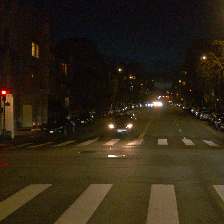
\includegraphics[width=0.15\textwidth]{figs/depth_prediction/DPT-1-ViT-22b-48459029-2/1_video.png}} \
    \subfigure{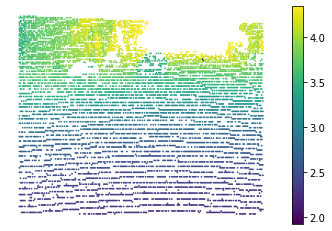
\includegraphics[width=0.2\textwidth]{figs/depth_prediction/DPT-1-ViT-22b-48459029-2/1_depth_scatter.png}} \
    \subfigure{
\includegraphics[width=0.2\textwidth]{figs/depth_prediction/DPT-1-ViT-L-50851792-2/1_predicted_depth_cbar.png}} \
    \subfigure{
\includegraphics[width=0.2\textwidth]{figs/depth_prediction/DPT-1-ViT-e-50851464-3/1_predicted_depth_cbar.png}} \
    \subfigure{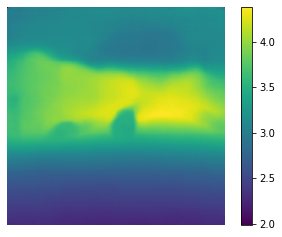
\includegraphics[width=0.2\textwidth]{figs/depth_prediction/DPT-1-ViT-22b-48459029-2/1_predicted_depth_cbar.png}}
    \subfigure{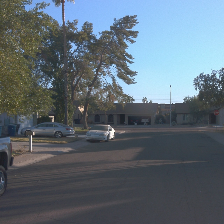
\includegraphics[width=0.15\textwidth]{figs/depth_prediction/DPT-1-ViT-22b-48459029-2/2_video.png}} \
    \subfigure{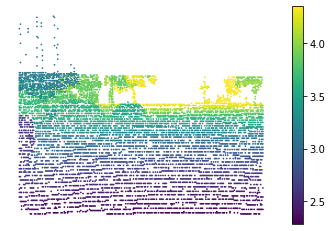
\includegraphics[width=0.2\textwidth]{figs/depth_prediction/DPT-1-ViT-22b-48459029-2/2_depth_scatter.png}} \
    \subfigure{
\includegraphics[width=0.2\textwidth]{figs/depth_prediction/DPT-1-ViT-L-50851792-2/2_predicted_depth_cbar.png}} \
    \subfigure{
\includegraphics[width=0.2\textwidth]{figs/depth_prediction/DPT-1-ViT-e-50851464-3/2_predicted_depth_cbar.png}} \
    \subfigure{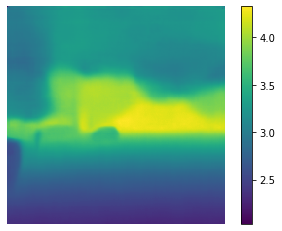
\includegraphics[width=0.2\textwidth]{figs/depth_prediction/DPT-1-ViT-22b-48459029-2/2_predicted_depth_cbar.png}}
    \addtocounter{subfigure}{-10}% reset counter to have columns a -- e.
    \subfigure[Input frame]{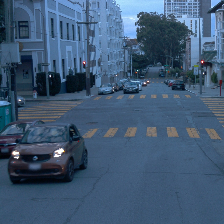
\includegraphics[width=0.15\textwidth]{figs/depth_prediction/DPT-1-ViT-22b-48459029-2/3_video.png}} \
    \subfigure[Sparse depth target]{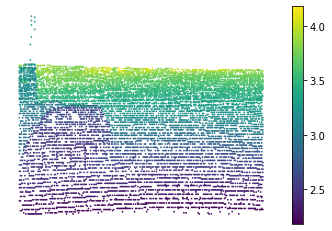
\includegraphics[width=0.2\textwidth]{figs/depth_prediction/DPT-1-ViT-22b-48459029-2/3_depth_scatter.png}} \
    \subfigure[DPT (ViT-L)]{
\includegraphics[width=0.2\textwidth]{figs/depth_prediction/DPT-1-ViT-L-50851792-2/3_predicted_depth_cbar.png}} \
    \subfigure[DPT (ViT-e)]{
\includegraphics[width=0.2\textwidth]{figs/depth_prediction/DPT-1-ViT-e-50851464-3/3_predicted_depth_cbar.png}} \
    \subfigure[DPT (ViT-22B)]{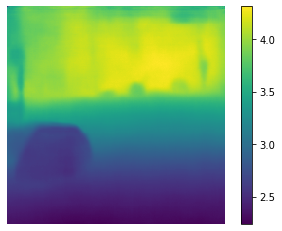
\includegraphics[width=0.2\textwidth]{figs/depth_prediction/DPT-1-ViT-22b-48459029-2/3_predicted_depth_cbar.png}}
    \caption{%\textbf
    {Monocular depth estimation}: (c, d, e) show estimated depth by a DPT head applied on ViT features, (a) shows the input frame and (b) shows the sparse ground-truth depth maps. Notice how (eg. in the third row) the model manages to go well beyond the available depth targets and makes what appear to be reasonable predictions for far-away cars, even though they are well out of LiDAR range. Ground-truth depth and depth predictions are visualized in $\log(1 + \text{depth})$ space.}
    \label{fig:dpt_depth_predictions_full}
\end{figure}

\begin{figure}[t!]
    \centering
    \subfigure{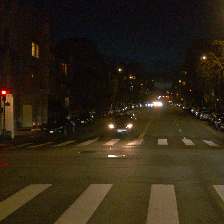
\includegraphics[width=0.15\textwidth]{figs/depth_prediction/DPT-1-ViT-22b-48459029-2/1_video.png}} \
    \subfigure{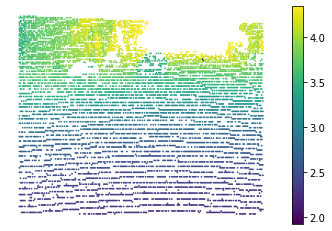
\includegraphics[width=0.2\textwidth]{figs/depth_prediction/DPT-1-ViT-22b-48459029-2/1_depth_scatter.png}} \
    \subfigure{
\includegraphics[width=0.2\textwidth]{figs/depth_prediction/DPT-1-ViT-L-50851792-2/1_predicted_depth_error_scatter.png}} \
    \subfigure{
\includegraphics[width=0.2\textwidth]{figs/depth_prediction/DPT-1-ViT-e-50851464-3/1_predicted_depth_error_scatter.png}} \
    \subfigure{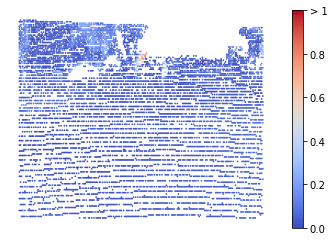
\includegraphics[width=0.2\textwidth]{figs/depth_prediction/DPT-1-ViT-22b-48459029-2/1_predicted_depth_error_scatter.png}}
    \subfigure{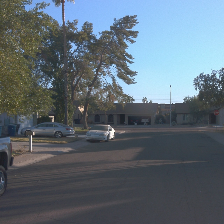
\includegraphics[width=0.15\textwidth]{figs/depth_prediction/DPT-1-ViT-22b-48459029-2/2_video.png}} \
    \subfigure{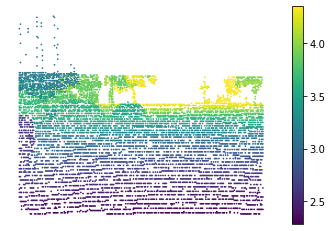
\includegraphics[width=0.2\textwidth]{figs/depth_prediction/DPT-1-ViT-22b-48459029-2/2_depth_scatter.png}} \
    \subfigure{
\includegraphics[width=0.2\textwidth]{figs/depth_prediction/DPT-1-ViT-L-50851792-2/2_predicted_depth_error_scatter.png}} \
    \subfigure{
\includegraphics[width=0.2\textwidth]{figs/depth_prediction/DPT-1-ViT-e-50851464-3/2_predicted_depth_error_scatter.png}} \
    \subfigure{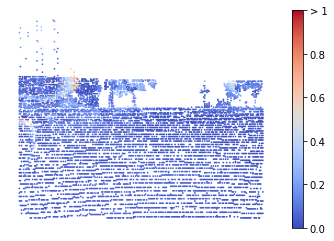
\includegraphics[width=0.2\textwidth]{figs/depth_prediction/DPT-1-ViT-22b-48459029-2/2_predicted_depth_error_scatter.png}}
    \addtocounter{subfigure}{-10}% reset counter to have columns a -- e.
    \subfigure[Input frame]{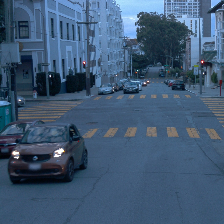
\includegraphics[width=0.15\textwidth]{figs/depth_prediction/DPT-1-ViT-22b-48459029-2/3_video.png}} \
    \subfigure[Sparse depth target]{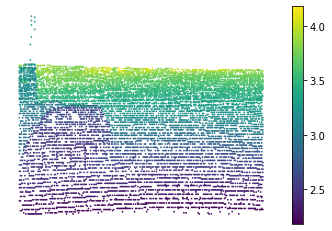
\includegraphics[width=0.2\textwidth]{figs/depth_prediction/DPT-1-ViT-22b-48459029-2/3_depth_scatter.png}} \
    \subfigure[DPT (ViT-L)]{
\includegraphics[width=0.2\textwidth]{figs/depth_prediction/DPT-1-ViT-L-50851792-2/3_predicted_depth_error_scatter.png}} \
    \subfigure[DPT (ViT-e)]{
\includegraphics[width=0.2\textwidth]{figs/depth_prediction/DPT-1-ViT-e-50851464-3/3_predicted_depth_error_scatter.png}} \
    \subfigure[DPT (ViT-22B)]{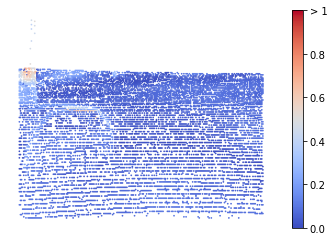
\includegraphics[width=0.2\textwidth]{figs/depth_prediction/DPT-1-ViT-22b-48459029-2/3_predicted_depth_error_scatter.png}}
    \caption{%\textbf
    {Monocular depth estimation errors}: (c, d, e) show absolute depth estimation errors by a DPT head applied on ViT features (for points where the ground truth is available), (a) shows the input frame and (b) shows the sparse ground truth depth maps. Notice how the outline of the car is clearly visible (light blue) from the sparse error maps in the third row when using ViT-L or ViT-e, while using \chonk leads to fewer errors in this region (darker blue). Ground-truth depth and absolute prediction errors are visualized in $\log(1 + \text{depth})$ space.}
    \label{fig:dpt_depth_predictions_full_error}
\end{figure}

\paragraph{Linear decoder.}

The linear decoder processes $16\times 16 \times 6144~$ ViT-22B feature maps using two transpose convolution layers of stride 2 and kernel size 5, followed by a $1\times 1$ convolution that outputs a low resolution depth map.
This is resized to $224\times 224$ using bilinear interpolation and clipped at $0$ to be valid predictions for $log\left(1 + \mathrm{depth}\right)$
The intermediate feature maps have $1536$ and $768$ dimensions each.
Linear activations are used in between layers so that the whole decoder is end-to-end linear.
This performed marginally better than a single $11\times 11$ stride $4$ transpose convolution layer, although the single layer decoder should be equally powerful in theory.
We suspect that this has to do with how hyper-parameters have been empirically optimized for smaller kernel sizes.

For the ViT-e and ViT-L baselines, the linear decoder is exactly the same except for a much smaller input feature dimension ($1792$ for ViT-e and $1024$ for ViT-L).
Thus the linear decoder on top of ViT-22B has more capacity than the same on top of ViT-e or ViT-l.
We controlled for this in two ways: (a) using a $1\times 1$ convolution on the ViT-22B features, we down-project them to $1792$ dimensions to match the feature map size of ViT-e, or (b) using a large hidden dimension ($4096$ in ViT-e's decoder and $6144$ in ViT-L's decoder) after the first convolution transpose layer, we approximately matched the number of parameters across the three models. In control (a), performance stayed roughly the same at $0.165$ relative absolute error (AbsRel) for ViT-22B. In control (b) performance for baselines did not change substantially in terms of relative absolute error, $0.208$ for ViT-e and $0.222$ for ViT-L. We therefore report results without these controls in~\cref{tab:depth_estimation}.

\subsubsection{Training Details}

We train the decoder for 300k steps with a batch size of 64 using Adam~\citep{kingma2014adam} and clip the gradients to a global norm value of 0.05 to stabilize training.
We linearly increase the learning rate for 2500 steps to 0.0002 (starting from 0) and then decay the learning rate with a cosine schedule~\citep{loshchilov2016sgdr} back to 0.

\subsubsection{Metrics}

We quantify performance using the following standard depth estimation metrics from the literature~\citep{hermann2020self, eigen2014depth}, and also report the MSE loss on the validation set:
AbsRel measures the mean absolute error between the ground truth and predicted depth relative to the ground truth, while the inlier fraction metrics ($\delta$) measure the fraction of valid pixels within a certain 
percentage
from ground truth.
All metrics were measured after undoing the log transformation.

\subsubsection{Qualitative Results}

We report qualitative depth predictions by DPT from different ViT backbones in \Cref{fig:dpt_depth_predictions_full}, and absolute prediction errors in \Cref{fig:dpt_depth_predictions_full_error}.